\documentclass[11]{article}
\usepackage[margin=1in]{geometry}
\usepackage{amsfonts,amsmath,amssymb}
\usepackage{fancyhdr}
\usepackage{graphicx}
\usepackage{float}
\usepackage{transparent}
\usepackage{eso-pic}
\usepackage[colorlinks,linkcolor={blue}]{hyperref}



\usepackage{listings}
\usepackage{color}


\definecolor{dkgreen}{rgb}{0,0.6,0}
\definecolor{gray}{rgb}{0.5,0.5,0.5}
\definecolor{mauve}{rgb}{0.58,0,0.82}

\lstset{frame=tb,
  language=Java,
  aboveskip=3mm,
  belowskip=3mm,
  showstringspaces=false,
  columns=flexible,
  basicstyle={\small\ttfamily},
  numbers=none,
  numberstyle=\tiny\color{gray},
  keywordstyle=\color{blue},
  commentstyle=\color{dkgreen},
  stringstyle=\color{mauve},
  breaklines=true,
  breakatwhitespace=true,
  tabsize=3
}



\newcommand\BackgroundPic{%
\put(0,0){%
\parbox[b][\paperheight]{\paperwidth}{%
\vfill
\centering
{\transparent{0.3} 
\includegraphics[width=\paperwidth,height=\paperheight,%
keepaspectratio]{background.png}}%
\vfill
}}}

\AddToShipoutPicture*{\BackgroundPic}

\pagestyle{fancy}
\fancyhead{}
\fancyfoot{}
\fancyhead[L]{\slshape \MakeUppercase{Notes}}
\fancyfoot[C]{\thepage}
%\renewcommand{\headrulewidth}{0pt}
\renewcommand{\footrulewidth}{0pt}

\parindent 0ex
\renewcommand{\baselinestretch}{1.5}

\begin{document}
\begin{titlepage}
\begin{center}
\vspace{1cm}
\Large{\textbf{Computer Science 101: Introduction to Java and Algorithms}}\\
\vfill
\line(1,0){400}\\
\huge{\textbf{Project 1: Game Of Life}}\\
\line(1,0){400}\\
\vfill
Erudition Labs\\
Computer Science 101: Introduction to Java and Algorithms\\
\today\\
\end{center}
\end{titlepage}

\tableofcontents
\thispagestyle{empty}
\clearpage
\setcounter{page}{1}
\section{John Conway`s Game of Life}
Most of this introduction comes from \url{<https://en.wikipedia.org/wiki/Conway\%27s_Game_of_Life>} If you would like to just read about it there. John Conway was a mathematician who was trying to create a simulation that would fit computer scientist, John von Neumann`s definition of what life is. Von Neumann was trying to do this by engineering a solution by making electromagnetic components randomly float in liquids or a gas. Another mathematician by the name of Stanislaw Ulam invented ``cellular automata`` to simulate what Von Neumann was trying to do. Finally, John Conway created a set of complex mathematical rules that would yield a configuration that would fit Von Neumann`s definition of life. That being said, Conway was more interested in trying to be able to complex and unpredictable cellular automatons that could go on forever or die out depending on the initial configuration. It`s and interesting way to see patterns evolve and show the emergence of organisms as well as their self-organization with Conway's deterministic rules.

\subsection{Cellular Automata}
Cellular automaton consists of a grid of cells that have a finite number of states and where rules are applied to all of the cells. It is quite commonly using in simulations in the sciences like physics, chemistry etc. We will be talking about how we will do this in a bit.

\subsection{The Rules}
Many conclusions have been drawn from Conway`s experiments. His mathematical rules can be summed up in words as the following.

We assume that we have an infinite 2d, orthogonal grid.

\begin{enumerate}
  \item Any live cell with fewer than two live neighbours dies, as if by underpopulation.
  \item Any live cell with more than three live neighbours dies, as if by overpopulation.
  \item Any dead cell with exactly three live neighbours becomes a live cell, as if by reproduction.
  \item Any live cell with two or three live neighbours lives on to the next generation.
\end{enumerate}

As it turns out, these rules, when applied to cellular automaton, will create complex patterns and form groups of cells (organisms) that do things like oscillating pulsation and even move.

\section{Our Project} 
We are going to implement this simulation using most of the concepts we have learned so far like variables, arrays, loops, if-statements and methods. We are going to translate the above descriptions and rules into working code.

\subsection{Modeling}
\subsubsection{2D infinite Grid and Cell States}
Lets think about how we can do this. The rules require an infinite 2d grid. Obviously, we cannot do the infinite part since we do not have infinite memory. However, we can still operate under the assumption that the grid is infinite.\\

We can use a two-dimensional array to represent our infinite 2d grid. We will need it to be fixed size, so we are going to have to break the rules a bit. When a cell is about to move past the limits of our 2d array, what are we going to do? Well one option is to wrap it around to the other side. However, I get a less infinite feeling form this. Another option, and the one we will most likely do, is to just kill the cell once is surpasses the confines of our grid.\\

So we have a 2d array to represent out 2d grid, and each element of our 2d array will be a ``cell``. In the rules, there are only two states that a cell can be in, alive or dead. There are a number of ways that we could represent those states. Perhaps we could use boolean values. If we create a 2d array of type boolean, then we could let ``true`` be ``alive`` and ``false`` be dead. This is probably the simplest way, but it is also limiting to two states. As we go through the course, we are going to be re-factoring this code as well as adding to it. I plan on adding to the rules and the sates. So to give us more options, we are going to use an integer array. This way, we can use ``0`` as dead and ``1`` as alive.\\

So again, we are going to represent our infinite 2d grid as a 2d integer array where once a cell leaves the confines of our array, we will simply assume that it will go on forever without really affecting our immediate system, so we will just kill that cell.

\subsubsection{Rules}
Now how can we apply the rules that govern that states of the cells. Well we could use a switch statement or if-statements to check each of the rules. We will loop over each element in our 2d array. Keep in mind that each element is a cell that is either dead or alive. We will use the current index to calculate where the neighbors of that cell is at. Then we will index into the array where the neighbor positions are to check their states. Finally, we will use their states to decide if the current cell should live or die. Once we have iterated over the entire array, that will be considered one generation.

\subsubsection{Visualization}
To Keep things simple, for now, we will simply be printing all of the live cells in the standard output, aka terminal. In other words, the simulation will be text based for now.

\subsubsection{UML Class Diagram}
UML stands for Universal Modeling Language. You may or may not learn this in an intro class, but if you plan on pursing software engineering, you will learn about this. There are many different types of diagrams for visualizing business requirements, sequencing out program flow, visualizing how the user interacts with the system, etc.  There is so many different diagrams that I don`t remember them all. However, they are particularly useful for organizing ideas and figuring out requirements for the product without ever having to write any code. This is a good idea if you are working with a client that knows nothing about programming. In this course we will be using the UML Class Diagrams to map out our code. In this case, we only have one class, but later will have more and we can use these diagrams to show how they all relate to each other.\\

\begin{figure}[H]
	\centering
	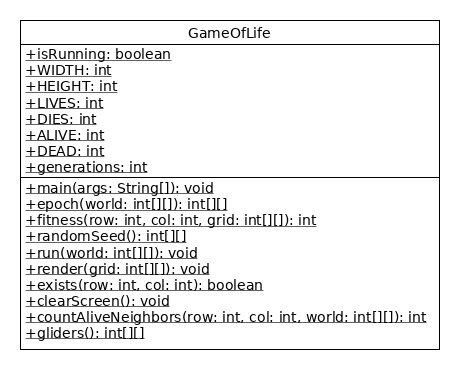
\includegraphics[scale=0.75]{classDiagram.png}
\end{figure}

Everything in the diagram has a purpose. The top part has the name of the class ``GameOfLife``. Under that is all the members of the class (we will learn more about what that means in later sections). Notice that we have the name of the variables and methods as well as their types and return types. The ``+`` means that these things are all public (``-`` is private and there are others). Finally, Notice that they are all underlined. Underlining means that they are static. So far, everything we will do will be static until we get to the classes sections.\\

If you would like to read more about these diagrams, checkout \url{<https://tallyfy.com/uml-diagram/>}

\subsubsection{Methods Overview}
\begin{itemize}
  \item \textbf{\textit{isRunning: boolean}} --
	This will be used to start and stop the program. Although at the moment we won`t be having a method to stop. I basically put this in there for future use.

  \item \textbf{\textit{WIDTH: int, HEIGHT int}} --
	When making global constant (aka final) variables, it is often good practice to capitalize all the letters in the name. These two variables will be used to define the size of the array that we will use to represent the world.
	
	  \item \textbf{\textit{LIVES: int, DIES:int, ALIVE: int, DEAD: int}} --
	These variables really serve no purpose other than to make the code more readable. Scattered throughout the code, we can talk about being alive or dead as 1 or 0, similarly we can talk about a cell getting to live or die by also using 1 and 0. So we can have a bunch of 1`s and 0`s everywhere and look at the rest of the condition to figure out what we are talking about in that particular spot, OR we can make named variables that make more sense as soon as we see it. It`s a good idea to opt in for better readability. 
	
	\item \textbf{\textit{generations: int}} --
	Used to keep count of how many times we have updated the world, simply for the sake of knowing because it can be interesting to see how long it takes for things to evolve.
	 \item \textbf{\textit{main}} --
	We have to have a main method.
	
	  \item \textbf{\textit{epoch(world: int[][])}} --
		In English, an epoch is just some moment in time where something meaningful happens. In our case, an epoch is basically a generation. An epoch will be applying the rules through one iteration of our 2d array 
	
	  \item \textbf{\textit{fitness(row: int, col: int, grid: int[][])}} --
	This method will look at a given cell in the 2d array. Once we have that cell it will look at all of it`s neighbors, and go through the game of life rules to determine if that cell will live or die.
	
	\item \textbf{\textit{randomSeed()}} --
	This method will will fill our 2d array with random living and dead cells.
	
		\item \textbf{\textit{run(world: int[][])}} --
	This is the driver of the game. Given a world, it will loop until we decide to kill the program, running the game.
	
		\item \textbf{\textit{render(grid: int[][])}} --
	Given a grid, this will print the world to the console screen.
	
		\item \textbf{\textit{exists(row: int, col: int)}} --
	Given the coordinates of the cell, this method will see if it is in the 2d array or not. If it`s not, then this will keep us from getting an ArrayIndexOutOfBounds exception.
	
		\item \textbf{\textit{clearScreen()}} --
	This just clears the console for the next epoch to be printed. Note that this only works in the terminal.
	
		\item \textbf{\textit{countLivingNeighbors(row: int, col: int, world: int[][])}} --
	Given a cell and the world, count all of the living neighbors. Note that Conway uses the 8 cell  Moore neighborhood. As opposed to the 4 cell  Von Neumann neighborhood.
	
		\item \textbf{\textit{gliders()}} --
		Puts some glider configurations into the 2d world.
\end{itemize}

\end{document}
